%!TEX root=../main.tex
\chapter{Climbing Mont Blanc Usability Goals}
This chapter starts with a definition of usable software systems in section \ref{sec:usability-def}. The section will define usability, and show aspects and characteristics in other \glspl{oj} which makes them usable with respect to the definition presented. Section \ref{sec:cmb-usability} ends the chapter with a discussion of usability goals for the \gls{cmb} system, aiming to make the system as usable as other acknowledged \glspl{oj}.

\section{Usability in Online Judge Systems}
\label{sec:usability-def}
Usability is defined in the ISO 9241 standard Part 11 as ``the extent to which a product can be used by specified users to achieve specified goals with effectiveness, efficiency and satisfaction in a specified context of use.'' \cite{ISO1998}. The definition is broad and covers many aspects of a product, or in our case a software system. A lot of research has been done in within software system usability, and literature seems to agree that the following five characteristics describe a usable software system \cite{holzinger2005, ferre2001}; \textit{learnability}, \textit{efficiency}, \textit{user retention over time}, \textit{error rate}, and \textit{satisfaction}. A quick summary of each characteristic found in literature is summarized below.

\paragraph*{Learnability:} The users ability to learn to use the system. This also involves the users ability to gain efficiency in using the system and reach their objectives in a quick manner.

\paragraph*{Efficiency:} Users should be allowed to obtain a high level of productivity when using the system. The usability is improved if the user are able to quickly reach their goals when using the system.

\paragraph*{User Retention Over Time:} The user should be able to return to the system after break from using it, and remember the core functionality of the system. A usable software system makes it easy to return into an efficient state without the need to learn the core functionality of the system anew. The characteristic is also refered to as \textit{memorability}.

\paragraph*{Error Rate:} The number of errors a users makes along the path of actions before reaching their goal. A low error rate among users improves the usability of the system.

\paragraph*{Satisfaction:} The users subjective thoughts about the system as well as making the system pleasant to use. This may involve functionality that is both visible and invisible through the system frontend. \\

Another related term to system usability is the notion of \textit{affordance} of things, which is defined by Donald Norman as ``the perceived and actual properties of the thing, primarily those fundamental properties that determine just how the thing could be used'' \cite{norman1988design}. Good affordances of entites and components in software systems will improve learnability, efficiency and user satisfaction while lowering error rates, and thereby improve the usability of the system. \\

The definition of \glspl{oj} as presented in section \ref{sec:related} is fairly simple. However, because of its simplicity, it is fairly important that the \gls{oj} is highly usable when users are actively using the system to solve programming problems. The most time consuming tasks done by most users in an \gls{oj}, at least in the \gls{cmb} system, is to read problem descriptions as well as submit code for automatic judgement. The time spent on reading and submitting is minimalistic compared to the time spent on developing code, and code development often happen off site in an offline environment if not explicitly offered by the \gls{oj}\footnote{Some of the mentioned \glspl{oj} has web based code editors, such as Kattis \cite{KATTIS} or HackerEarth \cite{HACKEREARTH}}. \\

Uploading code is one of the main actions done by users. Making the upload of code easy is important for both efficiency and learnability. \glspl{oj} like HackerEarth makes it easy to upload code, providing an online code editor which can compile and test the code or directly submit a solution like shown in Figure \ref{fig:hackerearth-upload}. The user also has the option of uploading source files directly, which makes it easier for the users wanting to submit source files instead of coding directly in the browser. Presenting multiple alternatives to the user, makes the user use the method he or she is most comfterable with. The upload feature also shows good affordance, and the user knows instinctively how to submit code. \\

\begin{figure}
    \centering
    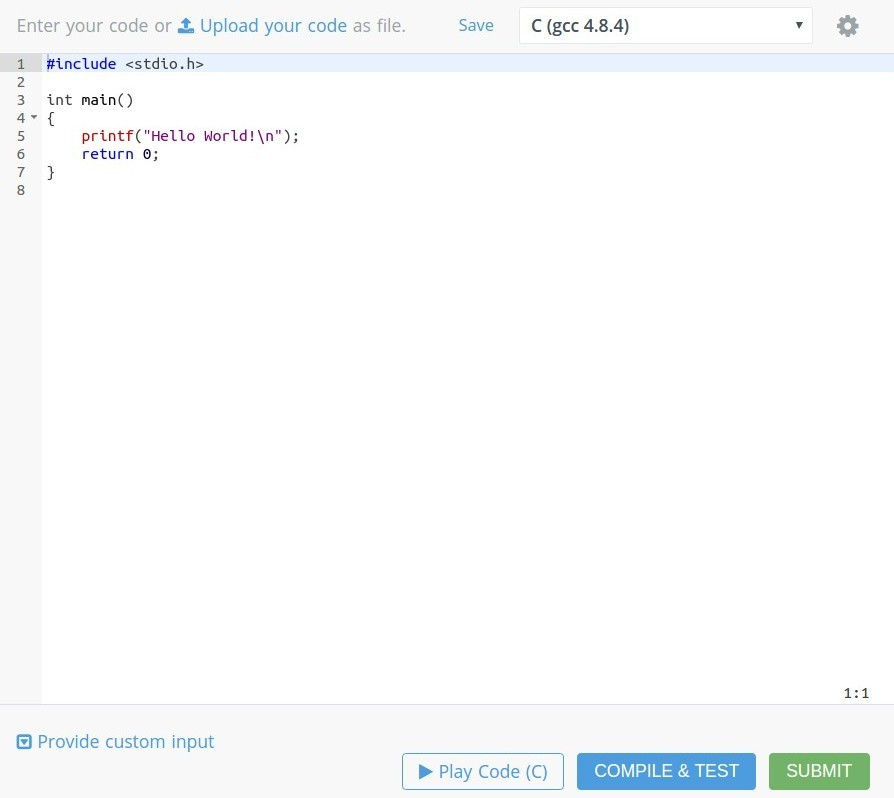
\includegraphics[width=0.8\textwidth]{figs/hackerearth_upload.jpg}
    \caption[HackerEarth Code Upload]{HackerEarth Code Upload (source: HackerEarth Website \cite{HACKEREARTH})}
    \label{fig:hackerearth-upload}
\end{figure}

It is also important that the user get feedback of the state of submitted program. Tracking the state and repeatedly report to the user whenever the state of the submission changes is important. It does not have to be very detailed, as long as the user get some notion of the state of the program. For example Kattis does not automatically report the state of a submitted program, but they displays a type of progress bar which is updated whenever test cases pases and the user manually refreshes the current view. However, the more information displayed about a submissions state the better, and . \\

Other features implemented by the judge should also behave as expected and the interface should be logically built. The \glspl{oj} presented in chapter offers various different features and going into depth about usability of this features is outside the scope of this thesis. However 

The different components in the user interface should also respond as expected and give logical feedback. Failing to do so might distract the user, and thereby blocking the user from reach his or hers goal.

In addition administrator users also needs a clean and usable admin interface. Usability in \glspl{oj} also involves making the system usable for system administrators and problem makers, and it is important that admin interface usage is simple and understandable. Usage of a given admin interface likely require some traning and knowledge about the system, but the interface should be simple so users do not have to read a manual every single time and quickly acheives high efficiency i.e high user retention over time.

\section{Climbing Mont Blanc Usability Goals}
\label{sec:cmb-usability}
Ease of use + performance + quick response + feedback
